\documentclass[11pt,a4paper,twoside]{book}

% ===== PACKAGES =====
\usepackage[utf8]{inputenc}
\usepackage[T1]{fontenc}
\usepackage{microtype}
\usepackage{amsmath,amssymb,amsthm}
\usepackage{graphicx}
\usepackage{xcolor}
\usepackage{tikz}
\usepackage{listings}
\usepackage{hyperref}
\usepackage{booktabs}
\usepackage{enumitem}
\usepackage{fancyhdr}
\usepackage{titlesec}
\usepackage{tcolorbox}
\usepackage{fontawesome5}
\usepackage{mdframed}

% ===== GEOMETRY - SMALLER MARGINS =====
\usepackage[
    top=2cm,
    bottom=2cm,
    left=2.5cm,
    right=2cm,
    marginparwidth=1.8cm,
    marginparsep=0.3cm,
    headheight=14pt,
    headsep=1cm,
    footskip=1cm
]{geometry}

% ===== COLORS =====
\definecolor{noteblue}{RGB}{13, 110, 253}
\definecolor{tipgreen}{RGB}{25, 135, 84}
\definecolor{importantorange}{RGB}{255, 149, 0}
\definecolor{warningyellow}{RGB}{255, 193, 7}
\definecolor{cautionred}{RGB}{220, 53, 69}
\definecolor{codegray}{RGB}{248, 249, 250}
\definecolor{linkblue}{RGB}{0, 123, 255}

% ===== HYPERREF SETUP =====
\hypersetup{
    colorlinks=true,
    linkcolor=linkblue,
    citecolor=linkblue,
    urlcolor=linkblue,
    bookmarksdepth=3,
    pdfborder={0 0 0}
}

% ===== GITHUB-STYLE CALLOUT BOXES =====
\tcbuselibrary{skins,breakable}

% Base style for all callouts - GitHub-like design
\tcbset{
    calloutbase/.style={
        enhanced,
        breakable,
        sharp corners,
        colback=white,
        colframe=#1,
        borderline west={3pt}{0pt}{#1},
        boxrule=1pt,
        left=12pt,
        right=8pt,
        top=8pt,
        bottom=8pt,
        fonttitle=\bfseries\sffamily\small,
        coltitle=#1,
        title style={left color=#1!10, right color=#1!5},
        before skip=1.5\baselineskip,
        after skip=1.5\baselineskip,
    }
}

% NOTE callout - Blue theme
\newtcolorbox{noteblock}{
    calloutbase=noteblue,
    colback=noteblue!3,
    title={\textcolor{noteblue}{\faInfoCircle}\ \textcolor{noteblue}{NOTE}}
}

% TIP callout - Green theme  
\newtcolorbox{tipblock}{
    calloutbase=tipgreen,
    colback=tipgreen!3,
    title={\textcolor{tipgreen}{\faLightbulb}\ \textcolor{tipgreen}{TIP}}
}

% IMPORTANT callout - Orange theme
\newtcolorbox{importantblock}{
    calloutbase=importantorange,
    colback=importantorange!3,
    title={\textcolor{importantorange}{\faExclamationCircle}\ \textcolor{importantorange}{IMPORTANT}}
}

% WARNING callout - Yellow theme
\newtcolorbox{warningblock}{
    calloutbase=warningyellow,
    colback=warningyellow!3,
    title={\textcolor{warningyellow!80!black}{\faExclamationTriangle}\ \textcolor{warningyellow!80!black}{WARNING}}
}

% CAUTION callout - Red theme
\newtcolorbox{cautionblock}{
    calloutbase=cautionred,
    colback=cautionred!3,
    title={\textcolor{cautionred}{\faExclamationTriangle}\ \textcolor{cautionred}{CAUTION}}
}
% ===== CODE LISTINGS - C LANGUAGE =====
\lstset{
    backgroundcolor=\color{codegray},
    basicstyle=\ttfamily\footnotesize,
    breakatwhitespace=false,
    breaklines=true,
    captionpos=b,
    commentstyle=\color{gray},
    frame=single,
    frameround=tttt,
    framesep=5pt,
    keywordstyle=\color{blue},
    language=C,
    numbers=left,
    numbersep=5pt,
    numberstyle=\tiny\color{gray},
    rulecolor=\color{black},
    showspaces=false,
    showstringspaces=false,
    showtabs=false,
    stringstyle=\color{red},
    tabsize=4,
    morekeywords={size_t, ssize_t, socklen_t, struct, typedef}
}

% ===== CHAPTER AND SECTION FORMATTING =====
\titleformat{\chapter}[display]
  {\normalfont\huge\bfseries\sffamily}
  {\chaptertitlename\ \thechapter}
  {20pt}
  {\Huge}
  
\titleformat{\section}
  {\normalfont\Large\bfseries\sffamily}
  {\thesection}
  {1em}
  {}
  
\titleformat{\subsection}
  {\normalfont\large\bfseries\sffamily}
  {\thesubsection}
  {1em}
  {}

% ===== HEADER AND FOOTER =====
\pagestyle{fancy}
\fancyhf{}
\fancyhead[LE]{\nouppercase{\leftmark}}
\fancyhead[RO]{\nouppercase{\rightmark}}
\fancyfoot[LE,RO]{\thepage}
\renewcommand{\headrulewidth}{0.4pt}
\renewcommand{\footrulewidth}{0pt}

% ===== THEOREM ENVIRONMENTS =====
\theoremstyle{definition}
\newtheorem{definition}{Definition}[chapter]
\newtheorem{example}{Example}[chapter]
\newtheorem{protocol}{Protocol}[chapter]

\theoremstyle{plain}
\newtheorem{theorem}{Theorem}[chapter]
\newtheorem{lemma}{Lemma}[chapter]

% ===== DOCUMENT METADATA =====
\title{Computer Networks: Course Reader}
\author{Computer Networks TAs et al.}
\date{Latest revision: \today}


% ===== OTHER =====
\setlength{\parindent}{0pt}
\setlength{\parskip}{0.5\baselineskip}
\setcounter{tocdepth}{1}
% link color dark blue
\hypersetup{
    linkcolor=blue,
    citecolor=blue,
    urlcolor=blue
}


\begin{document}

% ===== TITLE PAGE =====
\frontmatter
\maketitle

% ===== TABLE OF CONTENTS =====
\tableofcontents
% \listoffigures
% \listoftables

% ===== MAIN CONTENT =====
\mainmatter
\chapter{Preface}
\section*{Welcome to the CN Reader}
This reader was inspired by the wonderfully crafted Languages \& Machines reader - a course you will all take during your second year as a Computing Science student (at the time of writing this).

What follows is the \textbf{first edition} of this reader, so please be patient with us if we have made any mistakes and/or omissions.

The first edition was developed by Boyan Karakostov and Mihai David in 2025.

\begin{warningblock}
This reader should not be considered a replacement for lecture slides and tutorials. We strongly encourage you to attend all sessions provided by the course.
\end{warningblock}

\section*{How to Use This Reader}
This reader is designed to be a companion to the course, providing additional explanations, examples, and exercises. It is structured to follow the course syllabus, with each section corresponding to a topic covered in lectures.

\section*{Prerequisites}
This reader assumes basic familiarity with C programming and various computer science concepts. If you are new to C or need a refresher, consider reviewing introductory materials on C programming.

\section*{Feedback}
We welcome your feedback on this reader. If you find any errors, have suggestions for improvements, or would like to see additional topics covered, please reach out to the professor of this course or visit the reader's \href{https://github.com/Code-For-Groningen/CN-Reader}{GitHub repository}\footnote{For the paper readers: github.com/Code-For-Groningen/CN-Reader}.

\section*{License and Usage}
This reader is licensed under the \href{https://creativecommons.org/licenses/by-nc-sa/4.0/}{Creative Commons Attribution-NonCommercial-ShareAlike 4.0 International License}. You are free to share and adapt the material for non-commercial purposes, provided you give appropriate credit, indicate if changes were made, and distribute your contributions under the same license.

The code exerpts are licensed under GNU General Public License v3.0.

\section*{Updates and Errata}
This reader is a living document. We will periodically update it to correct errors, add new content, and improve clarity. Please check the \href{https://github.com/Code-For-Groningen/CN-Reader}{GitHub repository} for the latest version and any errata. The PDF provided by the course is a snapshot of the reader at the time of publication, and may not include the latest changes (but it will always be the most stable version).

If you'd like to report an error or suggest an improvement, please open an issue or submit a pull request on the GitHub repository. We appreciate your contributions to making this reader better for everyone.
\chapter{Introduction}
\section{Overview}
Computer Networks is a course that covers the fundamental concepts and technologies that enable communication between computers and devices. 

Understanding how data flows through networks, the protocols that govern this communication, and the architecture of network systems is not only essential for understanding modern computing but could also be pretty fun!

This course will explore various topics including:
\begin{itemize}
    \item The OSI and TCP/IP models
    \item Network protocols and standards
    \item IP addressing and subnetting
    \item Routing and switching
    \item Wireless networking
    \item Network security
\end{itemize}

For the practical component, we will be using Wireshark and Cisco Packet Tracer to analyze network traffic and simulate network configurations. There will be sections dedicated to guides as to how to set up and use these tools effectively.

Your practical assignments will involve programming in C \textbf{on Linux} to implement network protocols and other miscellaneous tasks.

\begin{importantblock}
Networking is handled differently depending on the operating system and C does not attempt to abstract this away. We implore you to check out why that is in detail, but for the purposes of this reader, this will be the only mention of it. The mandatory \textit{Operating Systems} course will cover some of the differences in more detail.

From here on out, we will assume you are using Linux or an equivalent Unix-like operating system. If you are using Windows, you will need to familiarize yourself with the \href{https://docs.microsoft.com/en-us/windows/wsl/install}{Windows Subsystem for Linux (WSL)} or use a virtual machine with a Linux distribution installed.
\end{importantblock}

\section{Setting Up Your Environment}

There are multiple tools and libraries that you will need to install to complete the practical assignments in this course. Follow the instructions below to set up your environment.

\subsection{Windows}
As mentioned earlier, for code, you will need to use the Windows Subsystem for Linux (WSL) or a virtual machine with a Linux distribution installed.

As for the tools, please download and install the following:
\begin{itemize}
    \item \href{https://www.wireshark.org/download.html}{Wireshark}
    \item \href{https://www.netacad.com/cisco-packet-tracer}{Cisco Packet Tracer}
\end{itemize}

\subsection{Linux}

\subsubsection{Debian-based systems (Ubuntu, Debian, Linux Mint)}\label{sec:debian-install}
For Debian-based distributions, you can install Wireshark using the package manager:
\begin{verbatim}
sudo apt update
sudo apt install wireshark
\end{verbatim}

\begin{noteblock}
Cisco Packet Tracer is not available in official repositories. Download it from the \href{https://www.netacad.com/courses/packet-tracer}{Cisco Networking Academy} website and follow their installation instructions.
\end{noteblock}

\subsubsection{Arch-based systems}
For Arch-based distributions:
\begin{verbatim}
sudo pacman -S wireshark-qt
\end{verbatim}

Cisco Packet Tracer can be installed from the AUR\@:
\begin{verbatim}
yay -S packettracer
\end{verbatim}

\subsection{macOS}
For macOS, you can install Wireshark using Homebrew:
\begin{verbatim}
brew install --cask wireshark
\end{verbatim}

Cisco Packet Tracer can be downloaded from the \href{https://www.netacad.com/courses/packet-tracer}{Cisco Networking Academy} website. While macOS is Unix-like, the C networking libraries should work \textbf{similarly to Linux}, though there may be minor differences in some system calls and headers.

\section{C Development Environment}

In addition to the networking tools above, you'll need a proper C development environment for the programming assignments.

\subsection{Essential Development Tools}

All systems will need:
\begin{itemize}
    \item A C compiler (GCC usually)
    \item Make build system
    \item A text editor or IDE
\end{itemize}

\subsubsection{Linux Installation}

On Debian-based systems:
\begin{verbatim}
sudo apt install build-essential git
\end{verbatim}

On Arch-based systems:
\begin{verbatim}
sudo pacman -S base-devel git
\end{verbatim}

\subsubsection{macOS Installation}

Install Xcode Command Line Tools:
\begin{verbatim}
xcode-select --install
\end{verbatim}

\subsection{Networking Libraries}

The assignments will use standard POSIX networking libraries that are included with your system:
\begin{itemize}
    \item \texttt{sys/socket.h} - Socket programming interface
    \item \texttt{netinet/in.h} - Internet address family
    \item \texttt{arpa/inet.h} - Internet operations
    \item \texttt{unistd.h} - POSIX operating system API
\end{itemize}

\begin{noteblock}
These are part of the standard C library on Unix-like systems.
\end{noteblock}
\chapter{OSI Layer Model}
\label{chap:osi}
% intro
\chapter{Introduction to OSI}\label{sec:osi_intro}
\section{What is OSI?}
\begin{figure}[h]
    \centering
    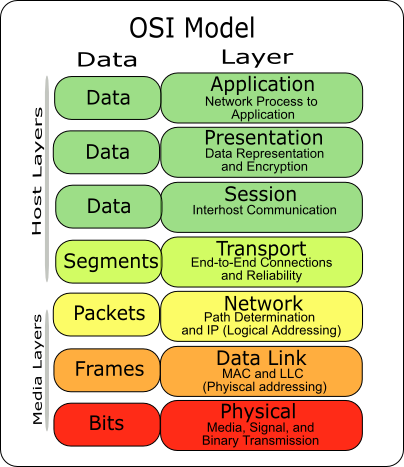
\includegraphics[width=.3\textwidth]{assets/osi/layers.png}
    \caption{The OSI Model Layers}\label{fig:osi_layers_intro}
\end{figure}
From chaos to order, the Open Systems Interconnection (OSI) model is a framework we use to understand how different networking protocols interact. Coincidentally (not so much), the Computer Networks course is structured around it.

\begin{table}[h]
    \centering
    \begin{tabular}{|c|c|c|}
        \hline
        \textbf{Layer} & \textbf{Function} & \textbf{Protocols} \\
        \hline
        Application & User interface & HTTP, FTP \\
        Presentation & Data translation & SSL/TLS \\
        Session & Session management & NetBIOS \\
        Transport & Data transfer & TCP, UDP \\
        Network & Routing & IP, ICMP \\
        Data Link & Node-to-node transfer & Ethernet \\
        Physical & Bit transmission & USB \\
        \hline
        \end{tabular}
    \caption{The Seven Layers of the OSI Model}\label{tab:osi_layers}
\end{table}

We will cover these layers by example in the next chapters, drilling down into layer-specific protocols and their intersections.


% physical layer
\section{Physical Layer}
\label{sec:osi_physical}

\vfill
\section*{tl;dr}
The first layer of the OSI model is responsible for the physical transmission of data over a medium. It defines the hardware elements involved in the communication process, such as cables, switches, and network interface cards (NICs). The physical layer ensures that data is transmitted as raw bits over a physical medium, without any concern for the content or meaning of those bits.

The Physical Layer is responsible for:
\begin{itemize}
    \item Converting bits to electrical, optical, or radio signals
    \item Defining voltage levels, timing, and physical data rates
    \item Specifying physical connectors and cable types
    \item Managing the physical topology of the network
    \item Synchronizing transmission between devices
\end{itemize}


\vfill
\subsection*{How does data exchange work? $\star$}
On a physics level, data exchange is about sending and receiving bits over some medium. 

This is done by converting the bits into electrical, optical, or radio signals. Electricity flows through wires, light pulses travel through fiber optics, and radio waves propagate through the air.


In essence, all of them boil down to a similar process: a change in some physical property (voltage, light intensity, or electromagnetic field) that can be detected by the receiving device, such that it can decode the signal back into bits. The process of converting bits into signals is called \textbf{modulation}, and the reverse process is called \textbf{demodulation}, while the process of converting bits into a specific format for transmission is called \textbf{encoding}.

\vfill
\newpage
\vfill
Let's look at a simple example of a 1-bit ADC (Analog to Digital Converter) that converts a voltage level into a bit value:

% assets/osi/physical/adc_plot.png
\begin{figure}[h]
    \centering
    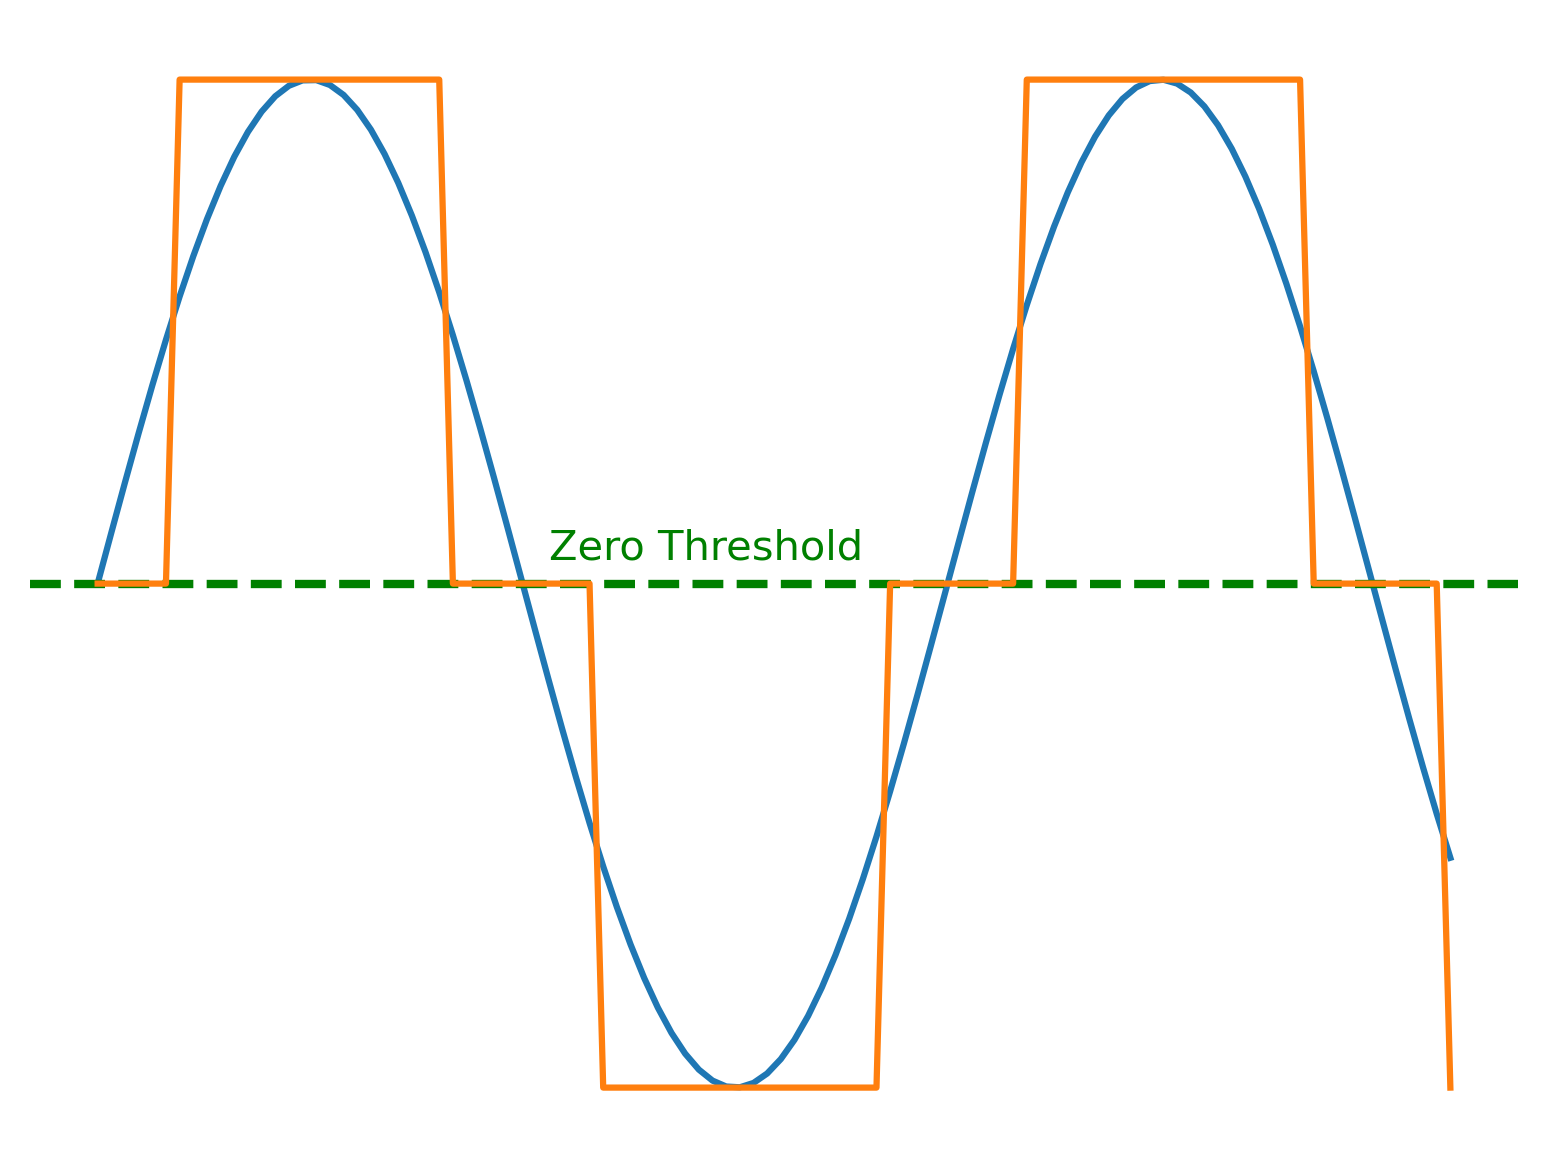
\includegraphics[width=.5\textwidth]{assets/osi/physical/adc_plot.png}
    \caption{Example of a 1-bit ADC converting voltage levels to bits}
    \label{fig:adc_plot}
\end{figure}

However, as you can probably guess, there are infinite ways for us to interpret this graph. It could correspond to \texttt{1010} or \texttt{1111000011110000} and so on. 
This is where clock signals come into play, which help us determine when to sample the signal and how to interpret it.

\vfill
\subsection*{Let's talk timing $\star$}
Clocks or timing signals are present in all hardware communication. 

The idea is to ensure that both sender and receiver are synchronized in their understanding of when bits are being sent and received. 

As an analogy, think of a dance where both partners need to be in sync to perform the moves correctly. If one partner is out of sync, the dance will look awkward and may not work at all.

\begin{figure}[h]
    \centering
    \begin{tikzpicture}
        % Clock signal
        \draw[thick] (0,2) -- (0.5,2) -- (0.5,3) -- (1,3) -- (1,2) -- (1.5,2) -- (1.5,3) -- (2,3) -- (2,2) -- (2.5,2) -- (2.5,3) -- (3,3) -- (3,2) -- (3.5,2) -- (3.5,3) -- (4,3) -- (4,2) -- (4.5,2);
        \node at (-0.5,2.5) {Clock};
        
        % Data signal
        \draw[thick] (0,0.5) -- (1,0.5) -- (1,1.5) -- (2,1.5) -- (2,0.5) -- (3.5,0.5) -- (3.5,1.5) -- (4.5,1.5);
        \node at (-0.5,1) {Data};
        
        % Sampling points
        \foreach \x in {0.5,1.5,2.5,3.5}
            \draw[red,thick] (\x,0.2) -- (\x,1.8);
        
        % Bit values
        \node at (0.5,0) {0};
        \node at (1.5,0) {1};
        \node at (2.5,0) {0};
        \node at (3.5,0) {1};
        
        % Labels
        \node at (2.25,-0.5) {Bit sampling occurs on clock transitions};
    \end{tikzpicture}
    \caption{Example rising edge clock synchronization}
    \label{fig:clock_sync}
\end{figure}
\vfill
\newpage
\section*{Transmission Media}
Different physical media carry the signals that transport our data across networks:

\subsection*{Guided Media}
Guided media confines signals to a specific path (literally "guided" along a cable or fiber). This includes:

\subsubsection*{Twisted Pair Cable}
You probably know this one well, as you find it in most local area networks (LANs) and telephone systems. It consists of pairs of insulated copper wires twisted together to reduce electromagnetic interference.

\begin{minipage}{0.6\textwidth}

UTP (Unshielded Twisted Pair) is the most common type, but there are also shielded variants like STP (Shielded Twisted Pair) and F/UTP (Foiled Unshielded Twisted Pair).

\end{minipage}
\hfill
\begin{minipage}{0.3\textwidth}
    \centering
    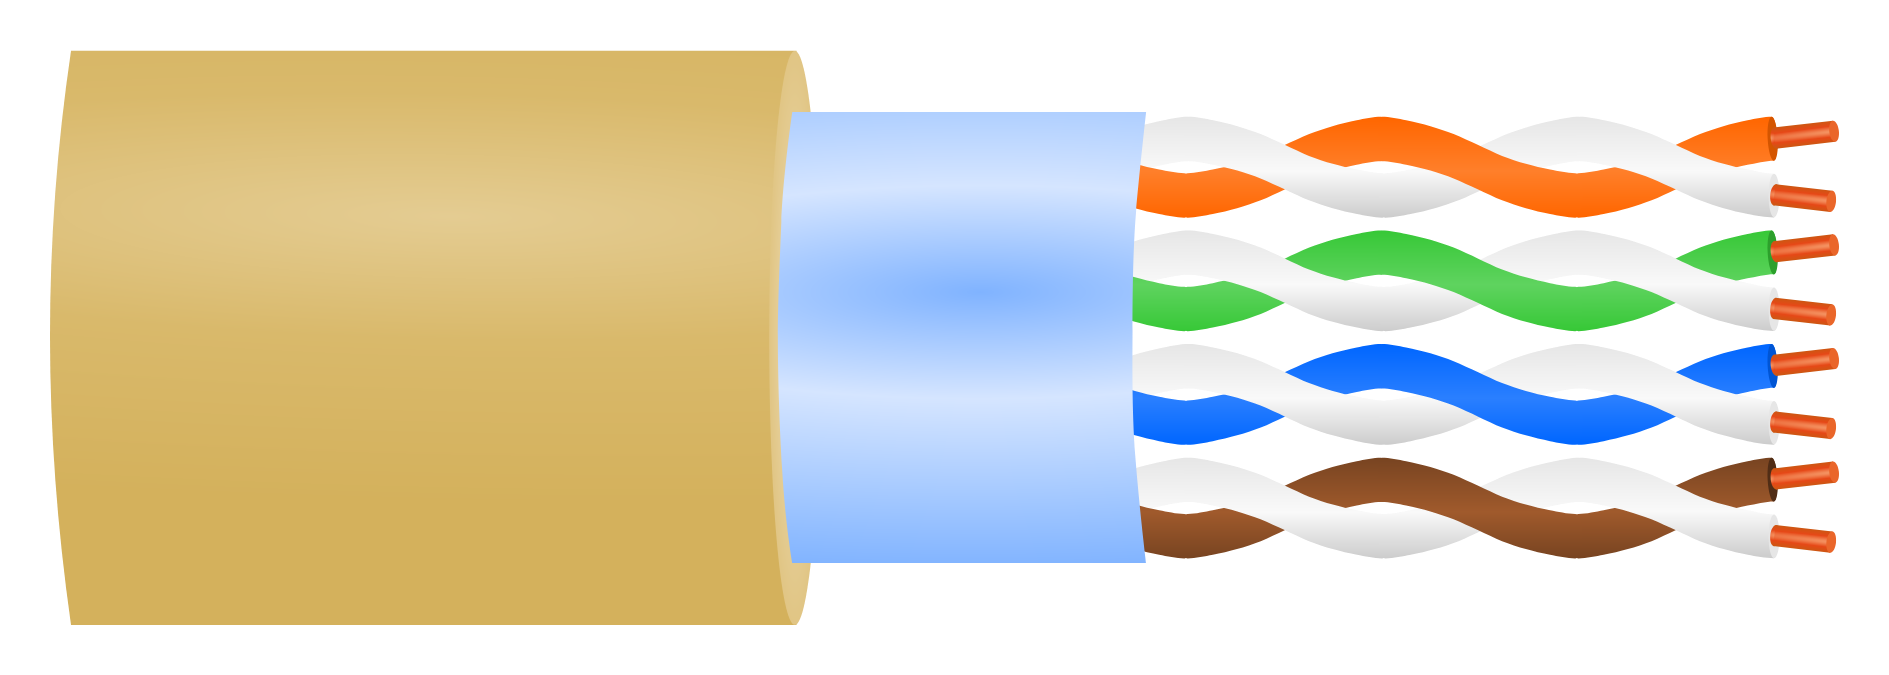
\includegraphics[width=\textwidth]{assets/osi/physical/f-utp.png}
    \caption{F-UTP (Foiled Unshielded Twisted Pair) example}
    \label{fig:twisted_pair}
\end{minipage}

\vspace{1em}

\subsubsection*{Coaxial Cable}
Usually used in cable television and broadband\footnote{Everything but dial-up.}.

\begin{minipage}{0.6\textwidth}

\vspace{0.5em}
\begin{itemize}
    \item Common in cable TV networks and was used in early Ethernet implementations
    \item Offers better noise immunity than twisted pair with higher bandwidth capacity, which is why radio amateurs still use it
\end{itemize}
\end{minipage}
\hfill
\begin{minipage}{0.3\textwidth}
    \centering
    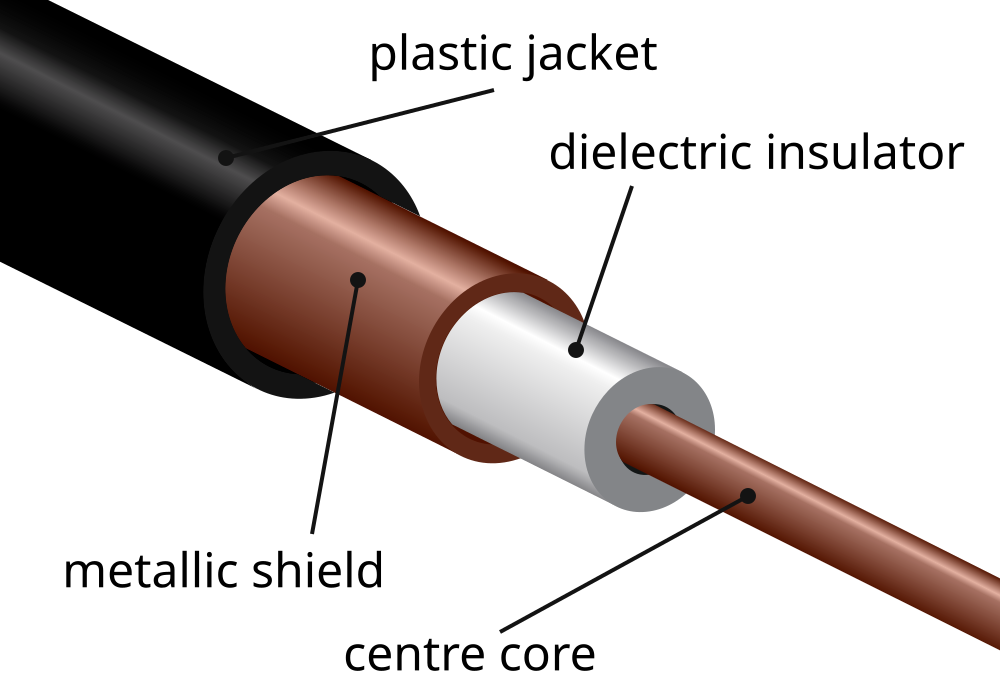
\includegraphics[width=\textwidth]{assets/osi/physical/coax.png}
    \caption{Coaxial cable structure}
    \label{fig:coaxial_cable}
\end{minipage}

\subsubsection*{Fiber Optic Cable}
Uses light to transmit data, making it the fastest and most reliable medium available today.

\begin{itemize}
    \item Composed of a core, cladding, and protective outer layer
    \item Immune to electromagnetic interference
    \item Supports high bandwidths
\end{itemize}

\begin{figure}
    \centering
    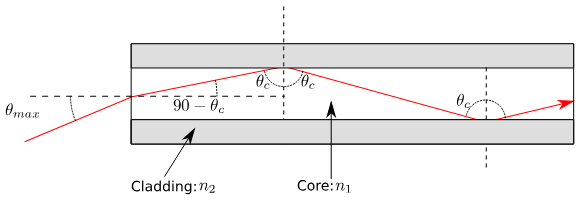
\includegraphics[width=.8\textwidth]{assets/osi/physical/fiber.png}
    \caption{Fiber optic cable structure}
    \label{fig:fiber_optic}
\end{figure}

\vspace{1em}

\newpage

\subsection*{Wireless Transmission}
Ever wondered how signals travel through the air? Different types of electromagnetic waves are used for wireless communication, each with its own characteristics.

% assets/osi/physical/spectrum.png
\begin{figure}[h]
    \centering
    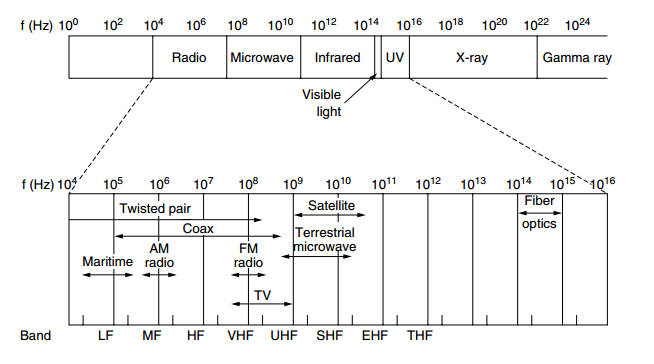
\includegraphics[width=.8\textwidth]{assets/osi/physical/spectrum.png}
    \caption{Electromagnetic spectrum showing different types of waves}
    \label{fig:em_spectrum}
\end{figure}

\subsubsection*{Radio Waves}
Radio waves are used for various wireless communication systems, including Wi-Fi, Bluetooth, and cellular networks. They can travel long distances (depending on wavelength) and penetrate through obstacles like walls.

\begin{noteblock}
    Fun fact! A lot of appliances like car remotes, thermostats and RC toys operate on the 433 MHz frequency band, which is a part of the radio spectrum. This is a perfect entry point if you'd like to hack your own devices or learn about radio communication.
\end{noteblock}

\subsubsection*{Microwaves}
Contrary to popular belief, microwaves are not just for cooking food. They are also used for point-to-point communication links, satellite communications, and some Wi-Fi networks. Microwaves have shorter wavelengths than radio waves, allowing them to carry more data, but faster attenuation\footnote{
    Attenuation: Reduction in signal strength as it travels through a medium, which can be caused by absorption, scattering, or reflection. 
    This is why we need repeaters/amplifiers!
} over distance.

\newpage
\section*{Standards and Specifications}
\subsection*{Ethernet Standards}
\begin{table}[h]
    \centering
    \begin{tabular}{|c|c|c|c|}
        \hline
        \textbf{Standard} & \textbf{Speed} & \textbf{Media} & \textbf{Distance} \\
        \hline
        10BASE-T & 10 Mbps & Cat3 UTP & 100m \\
        100BASE-TX & 100 Mbps & Cat5 UTP & 100m \\
        1000BASE-T & 1 Gbps & Cat5e UTP & 100m \\
        10GBASE-T & 10 Gbps & Cat6a UTP & 100m \\
        1000BASE-SX & 1 Gbps & Multi-mode fiber & 550m \\
        \hline
    \end{tabular}
    \caption{Common Ethernet Physical Layer Standards}
    \label{tab:ethernet_standards}
\end{table}

\subsection*{WiFi Standards}
\begin{itemize}
    \item 802.11a: 5 GHz, up to 54 Mbps
    \item 802.11b: 2.4 GHz, up to 11 Mbps
    \item 802.11g: 2.4 GHz, up to 54 Mbps
    \item 802.11n: 2.4/5 GHz, up to 600 Mbps
    \item 802.11ac: 5 GHz, up to 6.9 Gbps
    \item 802.11ax (WiFi 6): 2.4/5 GHz, up to 9.6 Gbps
\end{itemize}


% Modulation and encoding in physical layer
 testtesttest

% ===== APPENDICES =====
\appendix


\subsection*{@confestim - 28/07/25}
asdfds
\url{https://github.com/confestim/CN-Reader/pull/8}


% ===== BACK MATTER =====
\backmatter


\section*{Contributions}
\label{sec:contributions}
yo mama
\end{document}